\section{5. Linear Transformations}
% *********************************

\subsection{Introduction to linear transformations}
% =================================================

A \emph{transformation} or \emph{mapping} converts \underline{every} element in
the starting set (\textbf{domain}) to a \underline{unique} element in the arrival
sets (\textbf{codomain}). A transformation $T$ between spaces $V$ and $W$ is linear 
if and only if

\textbf{A)} $T(\mathbf{u} + \mathbf{v}) = T(\mathbf{u}) + T(\mathbf{v})$ and

\textbf{B)} $T(k\mathbf{u}) = kT(\mathbf{u})$

\subsubsection{Exercise 5.1.1}
%-----------------------------

Consider the transformation $T(\mathbf{u}) = \mathbf{Au}$. Determine $T(\mathbf{u})$
for the given \textbf{u}.

\begin{verbatim}
A= Matrix([[0, 1], [1, 0]])
u_a= Matrix([1, 3])
u_b= Matrix([-1, 5])
u_c= Matrix([sqrt(2), 1])
u_d= Matrix([-2, -3])

plt.rc('font', size= 8)
fig, ax= plt.subplots(1, 4)
for i, u in enumerate([u_a, u_b, u_c, u_d]):
    Tu= A.dot(u)
    ax[i].plot( (0, u[0]), (0, u[1]), color= 'blue', label= 'u' )
    ax[i].plot( (0, Tu[0]), (0, Tu[1]), color= 'red', label= 'T(u)' )
    ax[i].grid()

ax[0].legend(frameon= False)    
fig.set_size_inches(10, 2)
plt.savefig('figs/ex5_1_1a.pdf', bbox_inches='tight')
\end{verbatim}

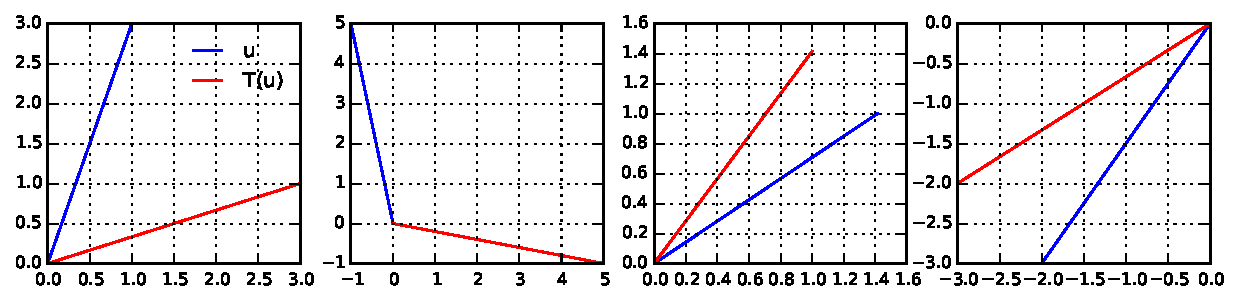
\includegraphics[width=1.2\linewidth]{figs/ex5_1_1a.pdf}

\subsubsection{Exercise 5.1.5}
%-----------------------------

Given the transformation (mapping) \ref{eq:ex5_1_5} in $\mathbb{R}^3$:

\begin{equation}\label{eq:ex5_1_5}
T{\left (\left[\begin{matrix}x\\y\\z\end{matrix}\right] \right )} =
\left[\begin{matrix}x + y\\
                    y + z\\
                    z + x\end{matrix}\right]
\end{equation}

determine whether the transformation \ref{eq:ex5_1_5} is linear.

In other words, we need to check whether the conditions \textbf{A} and
\textbf{B} above are satisfied.

First define a function with the transformation $T$ to be tested. Then define two generic
vectors \textbf{u} and \textbf{v} and see if applying $T$ satisfies the conditions
for linearity.

\begin{verbatim}
x, y, z, s, t, l, k= symbols('x y z s t l k', real= True)

def T(u):
    Tu= Matrix([u[0] + u[1],
                u[1] + u[2],
                u[2] + u[0]])
    return(Tu)
\end{verbatim}

Get two vectors and test conditions for linearity:

\begin{verbatim}
u= Matrix([x, y, z])
v= Matrix([s, t, l])

## Cond A:
assert (T(u + v)) - (T(u) + T(v)) == zeros(3, 1)

## Cond B:
assert (T(k * u) - k * T(u)).expand() == zeros(3, 1)
\end{verbatim}

Assertions return \texttt{True} hence the transformation \texttt{T} is linear.

Pay attention how the conditions for equality are tested in \sympy. We subtract
one term from the other and check the result is zero, in this case the zero vector
in $\mathbb{R}^3$ $[0\ 0\ 0]^T$. Using the double equal sign \texttt{==} would return
\texttt{False} in the second assertion since \texttt{==} tests for identity of form
not for \textbf{symbolic identity}. See also \href{https://github.com/sympy/sympy/wiki/Faq}{
Why does SymPy say that two equal expressions are unequal?}

The trasformation $T$:

$$
T(\left[\begin{matrix}x\\y\\z\end{matrix}\right]) = \left[\begin{matrix}\sqrt{x}\\\sqrt{y}\\\sqrt{z}\end{matrix}\right]
$$

Is not linear since $\sqrt{a + b} = \sqrt{a} + \sqrt{b}$ is not satisfied.

\begin{verbatim}
def T(u):
    Tu= Matrix([sqrt(u[0]), sqrt(u[1]), sqrt(u[2])])
    return(Tu)
    
u= Matrix([x, y, z])
v= Matrix([s, t, l])

## Cond A
(T(u + v)).expand() - (T(u) + T(v)).expand() == zeros(3, 1) ## False

## Cond B
(T(k * u)).expand() - (k * T(u)).expand() == zeros(3, 1) ## False
\end{verbatim}

\subsubsection{Exercise 5.1.6 a}
%-------------------------------

This is an helper function which might be useful elsewhere \footnote{See also
on StackOverflow \href{http://stackoverflow.com/questions/29434911/sympy-how-to-get-zero-for-absent-constant-term/}
{How to get zero for absent constant term.}}. Here we use it to implement the
tranformation \ref{eq:ex5_1_6a} where we need to swap the coefficients of a
polynomial. By returning a dictionary of terms and coefficients, \texttt{getCoeffDict}
makes the manipulation of coefficients easier.

\begin{equation}\label{eq:ex5_1_6a}
T(c_2 x^2 + c_1 x + c_0) = c_0 x^2 + c_1 x + c_2
\end{equation}

\begin{verbatim}
def getCoeffDict(exprs, x):
    """Return a dict of coefficients for each power of the variable `x` in
    expression `exprs`. Examples:
    
        >>> x, a, b, c= symbols('x a b c')
        >>> getCoeffDict(a*x**2 + b*x + c, x)
        {x**2: a, x: b, 1: c}
        >>> getCoeffDict(a*x**2, x)
        {1: 0, x: 0, x**2: a}
    """
    exprs= exprs.expand()
    n= Poly(exprs).degree(x)
    cdict= {}
    for i in range(0, n+1):
        cdict[x**i]= exprs.coeff(x, i)
    return(cdict)
\end{verbatim}

Let's proceede testing whether \ref{eq:ex5_1_6a} is a linear tranformation. Note
that the transformation \ref{eq:ex5_1_6a} works in polynomial space, not in
Euclidean space. However, the approach remains the same.

\begin{enumerate}
\item{Define the transformation of interest}
\begin{verbatim}
def T(p):
    k= getCoeffDict(p, x)
    Tp= k[1]*x**2 + k[x]*x + k[x**2]
    return(Tp)
\end{verbatim}

\item{Get two generic vectors:}
\begin{verbatim}
k= symbols('k', nonzero= True)
c0, c1, c2= symbols('c0 c1 c2')
b0, b1, b2= symbols('b0 b1 b2')

p= c2*x**2 + c1*x + c0
q= b2*x**2 + b1*x + b0
\end{verbatim}

\item Test condition $T(\mathbf{u + v}) = T(\mathbf{u}) + T(\mathbf{v})$
\begin{verbatim}
( (T(p+q)) - (T(p)+T(q)) ).expand() == 0 ## True
\end{verbatim}

\item Test condition $T(k\mathbf{u}) = kT(\mathbf{u})$
\begin{verbatim}
(T(k * p)) - (k * T(p)).expand() == 0 ## True
\end{verbatim}
\end{enumerate}

\subsubsection{Exercise 5.1.6 b}
%-------------------------------

Similar to \textit{a} above. For

$$
T(c_2 x^2 + c_1 x + c_0) = c_2^2 x^2 + c_1^2 x + c_0^2
$$

\begin{verbatim}
def T(p):
    k= getCoeffDict(p, x)
    Tp= k[x**2]**2 * x**2 + k[x]**2 * x + k[1]**2
    return(Tp)

p= c2*x**2 + c1*x + c0
q= b2*x**2 + b1*x + b0

# Is `kT(u) = T(ku)`?
((k*T(p)).expand() - (T(k*p)).expand()) == 0 # False
\end{verbatim}

Condition $T(k\mathbf{u}) = kT(\mathbf{u})$ can't be satisfied hence the
transformation is not linear.

$$
k \left(c_{0}^{2} + c_{1}^{2} x + c_{2}^{2} x^{2}\right) \neq c_{0}^{2} k^{2} + c_{1}^{2} k^{2} x + c_{2}^{2} k^{2} x^{2}
$$

\subsubsection{Exercise 5.1.7 a}
%-------------------------------

Check whether matrix transposition is a linear transformation. See \texttt{?Matrix.equals}
for testing matrix equality.

\begin{verbatim}
def T(A):
    return A.transpose()

a, b, c, d, e, f, g, h, i= symbols('a:i')
A= Matrix(2,2, [a,b,c,d])
B= Matrix(2,2, [f,g,h,i])

T(A+B).equals(T(A) + T(B)) ## True
(k*T(A)).equals(T(k*A))    ## True
\end{verbatim}

Matrix transposition \emph{is} linear.

Again, we are not working in Euclidean space but the approach is the same. This
is \emph{matrix space of size \emph{n} by \emph{n}}.

\subsubsection{Exercise 5.1.9}
%-------------------------------

Test whether \emph{integration} is linear. Note that integration maps from space
$C{0, 1}$ to $\mathbb{R}$.

\begin{verbatim}
f= Function('f')(x)
def T(f):
    return integrate(f, (x, 0, 1))
    
x= symbols('x', real= True, nonnegative= True, nonzero= False)
f= Function('f')(x)
g= Function('g')(x)

(T(f+g)).equals(T(f) + T(g)) ## Returns None
(k*T(f)).equals(T(k*f))  ## True
\end{verbatim}

First condition is satisified since:

$$
\int_{0}^{1} f{\left (x \right )} + g{\left (x \right )}\, dx = \int_{0}^{1} f{\left (x \right )}\, dx + \int_{0}^{1} g{\left (x \right )}\, dx
$$

\sympy returns \texttt{None} and this might be ok since \emph{$[$\texttt{Function.equals} returns$]$ None
(instead of T/F) for an expression that *is* zero but won't simplify to zero.}
(See \href{https://groups.google.com/forum/#!topic/sympy/xP_uM49pXeo}{\sympy discussion group})